\customHeader{1}{Tokenization and Embeddings}
\label{02_tokenization_and_embeddings}

Most \gls{nlp} tasks for text start with a corpus of documents. The documents may have been manually collected by humans; automatically collected, for example, using web scrapping tools, generating text from templates, or, most recently, sampling outputs from \gls{ai} tools like GPT-3 \myparencite{wang-etal-2021-want-reduce} and ChatGPT \myparencite{huang2023chatgpt}; or constructed using a mixture of human and automatic input.

Given that natural language is always evolving, the first step in \textclassification{} is to determine the Vocabulary that the system will use. \emph{\tokenization{}} is the process of breaking text into smaller components, called \emph{tokens}. As a first approach, one may use the intuitive idea of \emph{word} for tokens, in languages with a morphosyntax similar to English (Figure \ref{fig:naive_tokenization}). The collection of unique tokens derived from a text corpus constitutes the Vocabulary.

\begin{figure}
    \centering
    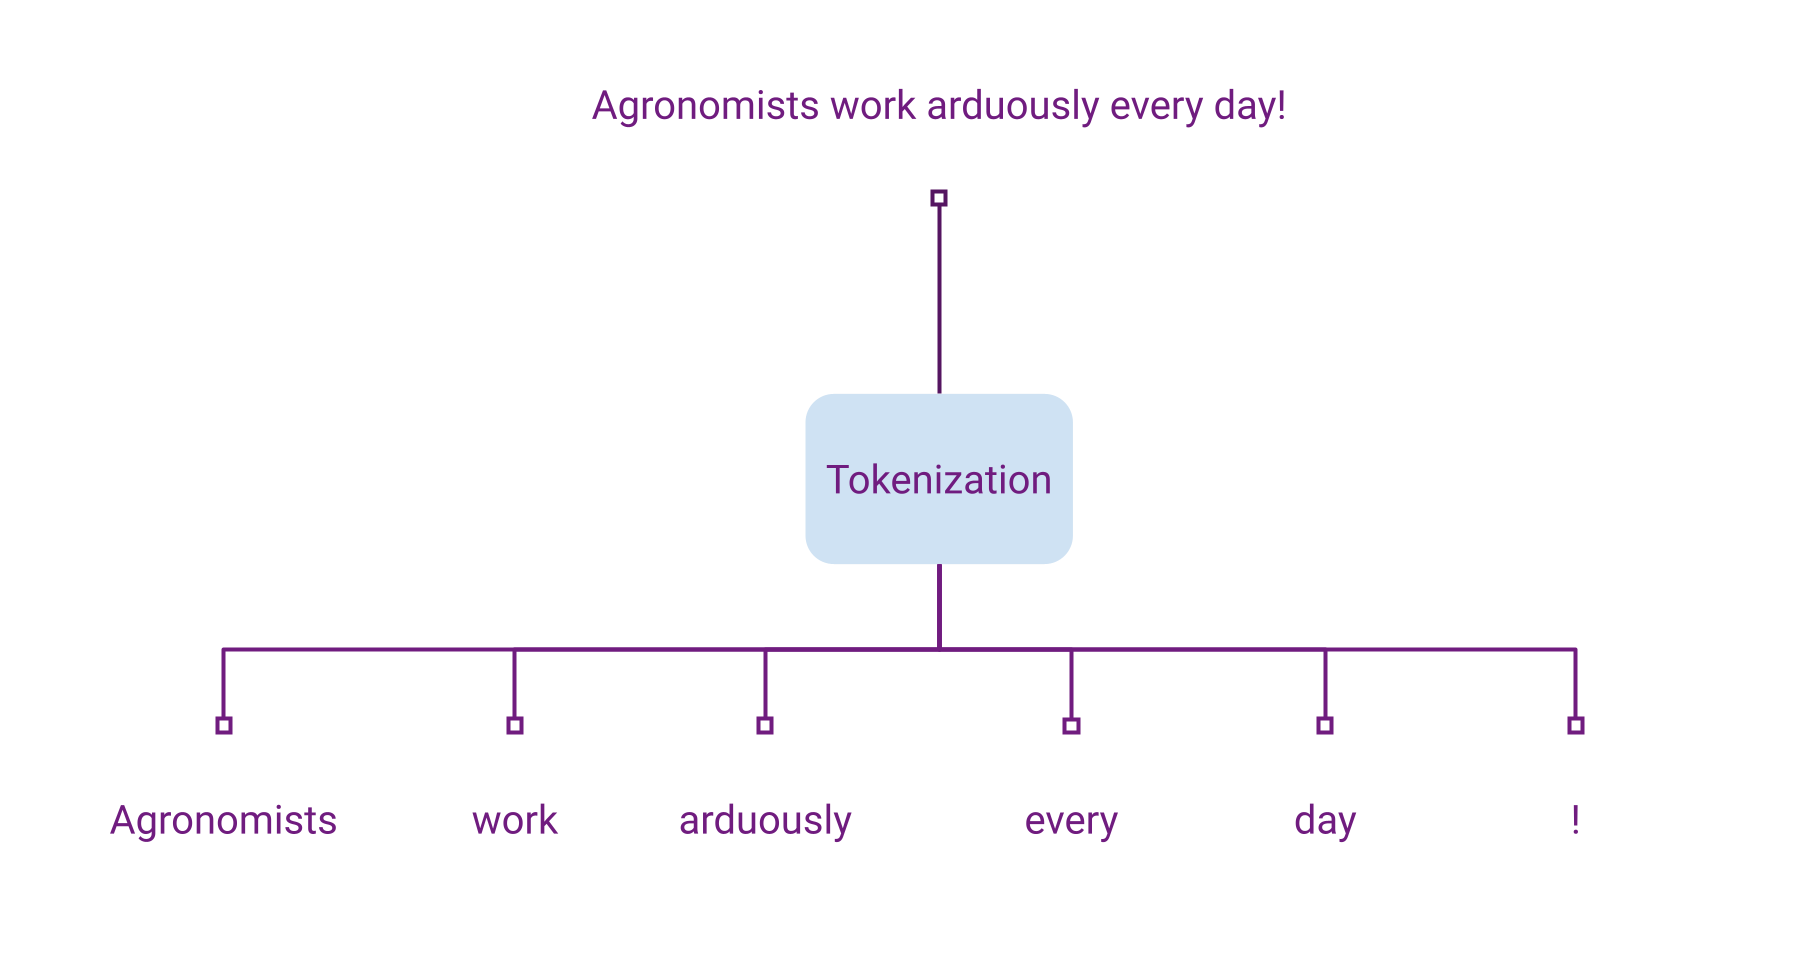
\includegraphics[width=0.75\textwidth]{Figures/02/01_Naive_Tokenization.png}
    \caption{Naive tokenization}
    \label{fig:naive_tokenization}
\end{figure}

However, naive word tokenization\footnote{Another simple tokenization technique is \emph{character-level tokenization}, where text is simply divided into its characters. This tokenization technique falls outside the scope of this work.} quickly runs into out-of-vocabulary (OOV) words when presented with new data. More recently, it has been found advantageous to work with \emph{subword units}. This approach aims to handle out-of-vocabulary (OOV) words by splitting them into smaller units. For example, in English, one may take affixes as subwords (\texttt{pre-}, \texttt{-ing}, \texttt{-ed}, etc...), which may improve the \gls{nlp} system's handle of morphology. Nevertheless, rather than manually defining rules for splitting words into subwords, there are two popular frequency-based algorithms for creating this type of tokenizer:

\begin{itemize}
    \item \emph{\gls{bpe}} \myparencite{sennrich2015neural} builds a vocabulary by iteratively merging the most frequent pair of characters or character sequences in a given text corpus. It starts with a character-level vocabulary and merges the most frequent pair of tokens until a desired vocabulary size is reached.
    \item \emph{\gls{wp}} \myparencite{wu2016google} begins by creating a vocabulary that consists of all the characters found in the training data. It then proceeds to learn a specific number of merge rules. Unlike \gls{bpe}, \wordpiece{} Tokenization selects symbol pairs that maximize their frequency relative to its constituent symbols, rather than choosing the most frequent symbol pair.
\end{itemize}

Usually, these algorithms produce different tokenizations of the same text, and thus, different vocabularies. Figure \ref{fig:02_tokenizer_comparison} shows a sample output from the \gls{wp} implementation in \mytextcite{BERT_paper} and the \gls{bpe} implementation in \mytextcite{roberta} for English text.

\begin{figure}
    \centering
    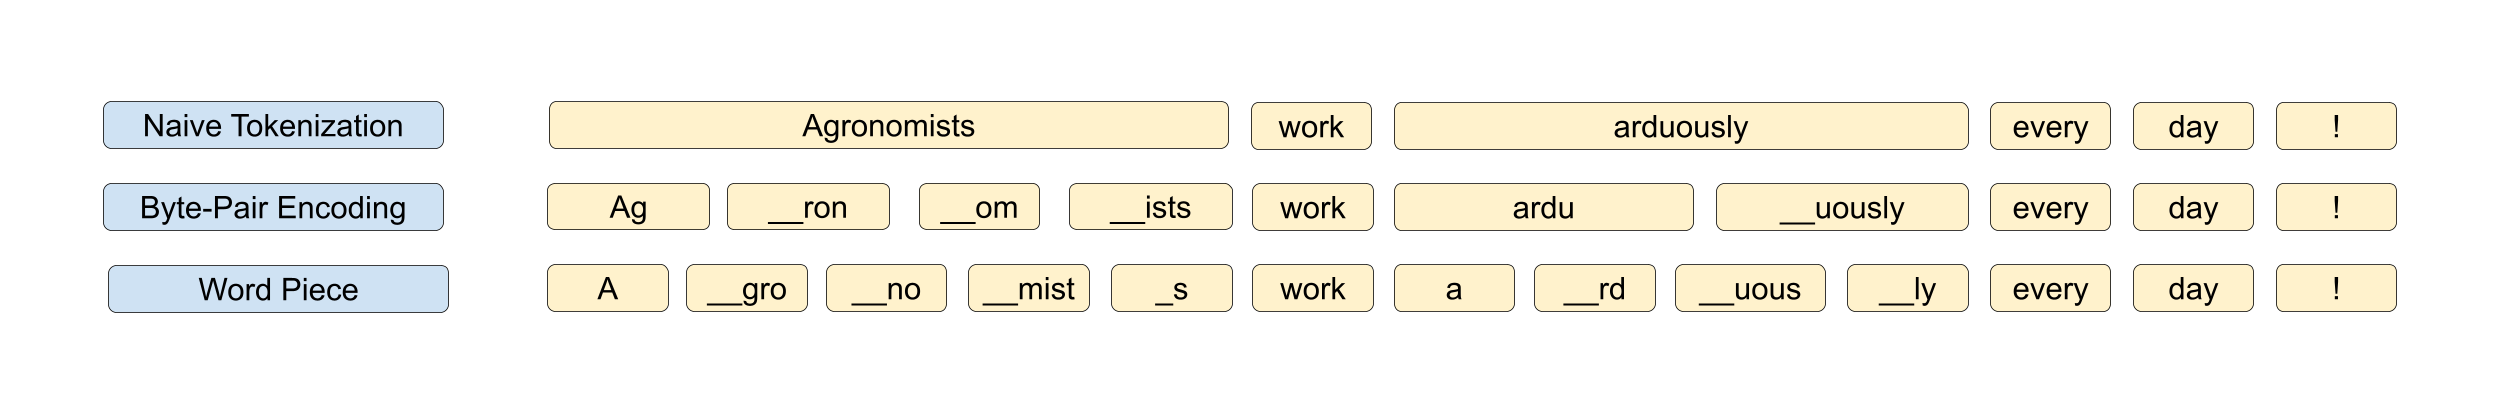
\includegraphics[width=\textwidth]{Figures/02/02_Tokenizer_comparison.png}
    \caption{Different tokenization approaches: naive, \bpe{}, and \wordpiece{}}
    \label{fig:02_tokenizer_comparison}
\end{figure}

Even though there are \textclassification{} approaches which only consider the distribution of tokens in a corpus, like \emph{Naive Bayes Classification} \myparencite{statistical_nlp_naive_bayes}, recent breakthroughs in \gls{nlp} have been enabled by \emph{text embeddings}, which are vector representations of text in high-dimensional space. They are intended to capture the semantic and syntactic relationships between texts, allowing computational models to understand and manipulate textual data. Word embeddings are a type of text embeddings that assign a vector representation to each token in a text. 
Typically, embeddings serve as \emph{input features} for textual data, which are then fed into \gls{ml} algorithms (Figure \ref{fig:02_embeddings_for_training_classification}).
While word embeddings are widely used, \textclassification{} specifically benefits from the use of \emph{document embeddings}. Document embeddings assign a vector to each entire document, allowing for more comprehensive analysis and classification of texts based on their overall content and context. Intuitively, text embeddings represent text with similar meaning close to each other and far away from texts with different meanings (Figure \ref{fig:word_and_document_embeddings}).

\begin{figure}
    \centering
    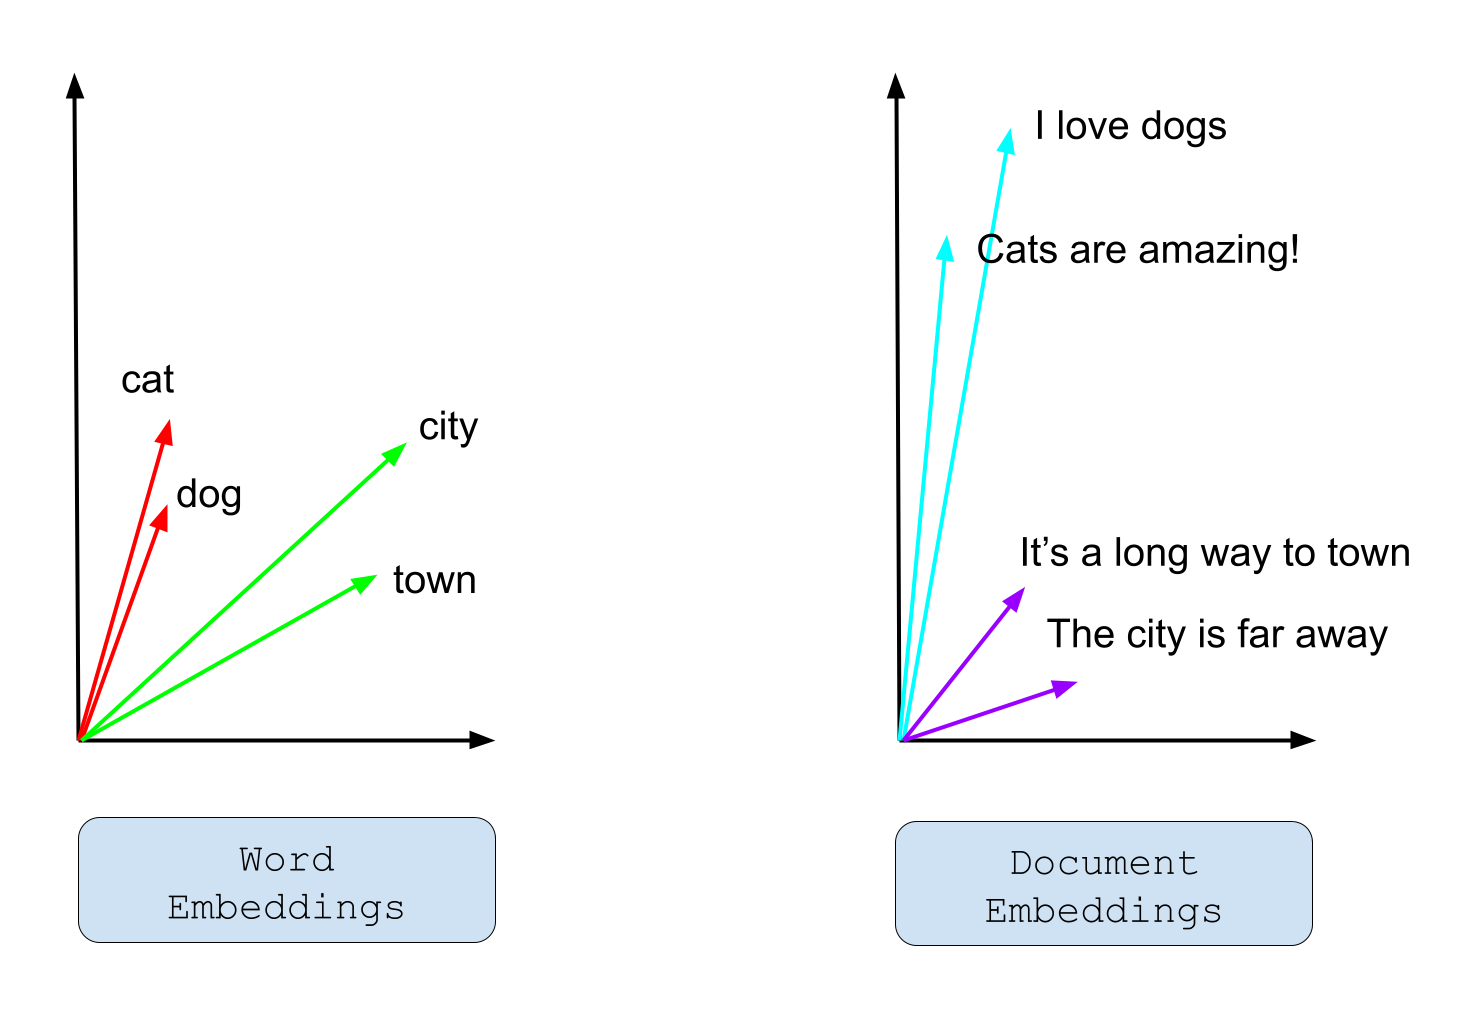
\includegraphics[width=0.75\textwidth]{Figures/02/02_embeddings.png}
    \caption{Word and Document embeddings}
    \label{fig:word_and_document_embeddings}
\end{figure}

\begin{figure}
    \centering
    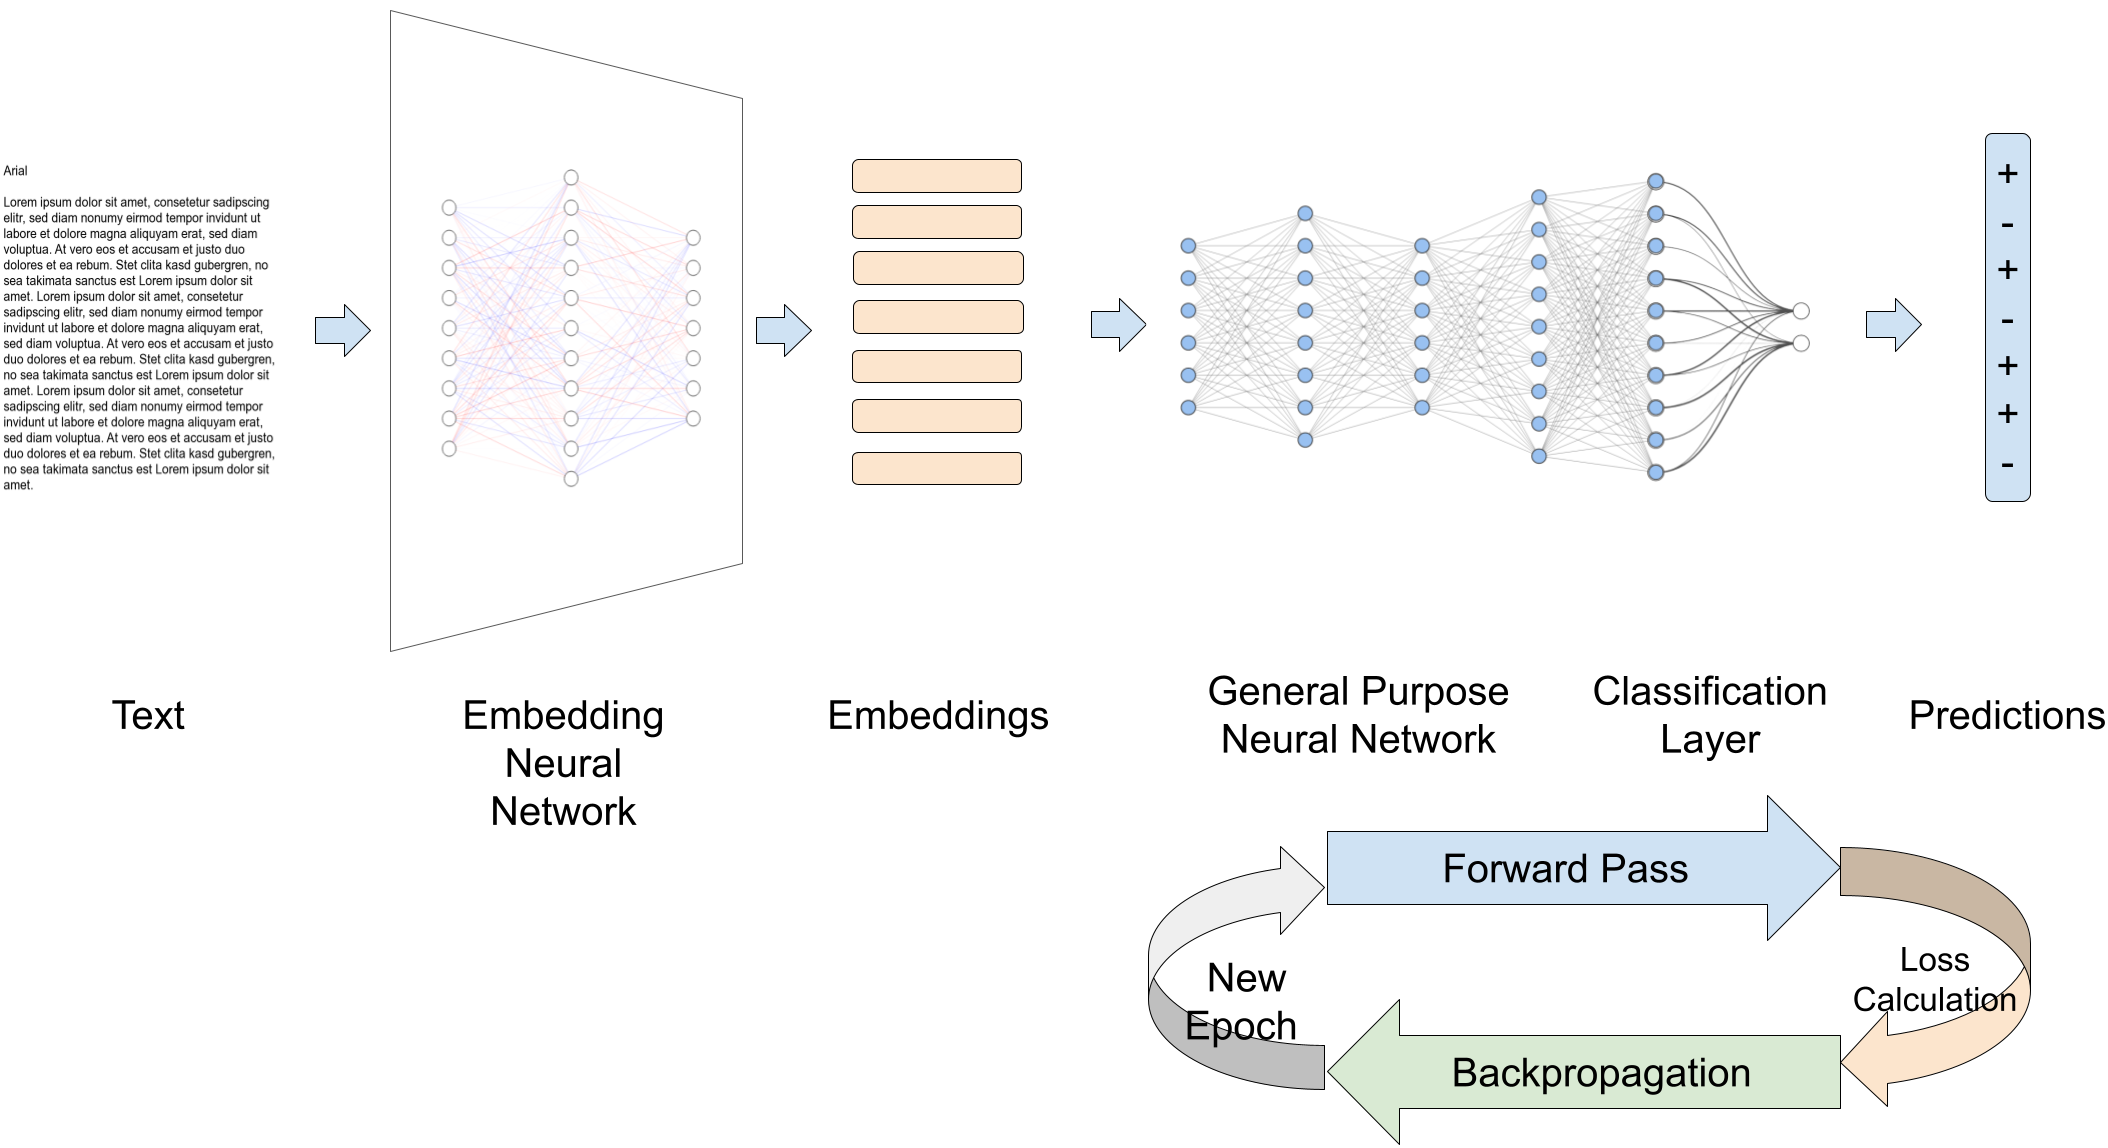
\includegraphics[width=0.9\textwidth]{Figures/02/02_nns_for_nlp.png}
    \caption{Using Embeddings to train Neural Networks for Classification}
    \label{fig:02_embeddings_for_training_classification}
\end{figure}

Text embeddings have undergone significant evolution over the years, with several techniques and models contributing to their development. We present a brief overview of the key milestones in the evolution of word embeddings:

\begin{itemize}
    \item Early approaches focused on frequency-based representations, such as Bag-of-Words (BOW) one-hot encoding\footnote{A one-hot vector has all its components null, except one which has value one} and term frequency-inverse document frequency (TF-IDF). These methods assigned weights or binary values to words based on their occurrence in the corpus, without capturing semantic relationships.
    \item \emph{Word2Vec} \myparencite{mikolov2013linguistic} popularized the concept of word embeddings trained using unsupervised learning. These models utilized shallow neural networks to learn word embeddings by predicting neighboring words or contexts. 
    \item \emph{GloVe} embeddings \myparencite{pennington-etal-2014-glove}  were trained on word co-occurrence statistics from a large corpus. It leveraged both global word co-occurrence information and local context windows to create meaningful vector representations.
    \item \gls{rnn} architechtures, such as GRU (Gated Recurrent Unit), LSTM (Long Short-Term Memory),  and Bi-LSTM (bidirectional LSTM), provided a breakthrough in capturing sequential dependencies and long-term dependencies within sentences, for example with \emph{InferSent} document embeddings \myparencite{infersent_bilstm}. By processing sentences sequentially, \gls{rnn}s generated fixed-dimensional vector representations at the sentence level. However, they faced challenges with long-term dependencies and were computationally expensive for longer sentences.
    
    \item  Contextualized word embeddings introduced the idea of generating word representations that varied depending on the context in which they appeared. Models like \emph{ElMo} (Embeddings from Language Models) \myparencite{elmo} and OpenAI's GPT (Generative Pre-trained Transformer) \myparencite{gpt} employed deep contextualized models and transformers to produce dynamic word embeddings.
    \item Transformer models, including Google's \BERT{} (Bidirectional Encoder Representations from Transformers) \myparencite{BERT_paper}, OpenAI's GPT-2 \myparencite{gpt2} and GPT-3 \myparencite{gpt3}, revolutionized the field by leveraging attention mechanisms and large-scale pre-training. These models introduced contextualized word embeddings on a larger scale and achieved state-of-the-art performance across various NLP tasks. The \BERT{} family of models has gained significant popularity due to its ability to efficiently generate contextualized embeddings for both individual tokens and entire documents at a low cost. Due to this factor, they will serve as primary tools in this project.
\end{itemize}

After tokenizing documents and calculating embeddings we transform textual data into a spatial representation apt for computation, and thus we can leverage the power of Neural Networks for \textclassification{}, which we proceed to explain in the next section.
